\documentclass{beamer}

\usetheme{simple}

\usepackage{lmodern}
\usepackage[scale=2]{ccicons}

% TODO: 
%   position adjustement
%   change colours
%       

% Watermark background (simple theme)

%\setwatermark{\includegraphics[height=8cm]{img/Heckert_GNU_white.png}}


\title{}
\subtitle{STLCutter.jl}
\date{\today}
\author{Pere Antoni Martorell}
\institute{\url{http://github.com/pmartorell/STLCutters.jl}}

\begin{document}

\maketitle
\begin{frame}{Performed tests}

  Experiments from issue
  \href{https://github.com/pmartorell/STLCutters.jl/issues/11}{\#11}

  \vfill{}

  \begin{columns}[c]

    \column{.45\textwidth}
    \textbf{3. Thingi 10k dataset}

    Filtered
    \href{https://ten-thousand-models.appspot.com/results.html?q=is+closed\%2C+is+oriented\%2C+is+manifold\%2C+is+not+degenerate\%2C+without+self-intersection\%2C+\%23df\%3D0}{\underline{5k geometries}}
    with quality criteria (closed,oriented,non degenerate...)

    Tests:
    \begin{itemize}
      \item
        Background mesh: 100 cells in largest direction
      \item
        Gadi, Titani (HPCs)
    \end{itemize}
    
    
    \column{.45\textwidth}
    \textbf{1.1,2.1. Robustness Matrix}

    Matrix axis:
    \begin{itemize}
      \item
        13 geometries
      \item
        6 background mesh h-refinements: \texttt{14*2\^(0:5)}
      \item
        1 origin + 17 displacements + 17 rotation : \texttt{10\^(-17:-1)}
    \end{itemize}

  \end{columns}
\end{frame}


\begin{frame}{Thingi 10k dataset}
  \framesubtitle{Few numbers}

  Num geometries: 5052

  Not available: 312 (6.2\% of total)

  Load error: 7 (0.14\% of total)

  Available: 5052-312-7=4733 (93.7\% of total)

  \textbf{Success geometries:} 3817 (78.5\% of available, 97.4\% of launched)

  Large volume error ($>$1e-14): 67 (1.8\% of success) (100\% due to small facets)

  Found to be degenerated: 4

  Failed: 34 (0.89\% of success)

  Missing (running): 916 (19.4\% of total)
  \vfill{}
  \textbf{ONGOING:}
  Try to fix problems with small facets
  Indentify failed runs as degenerate or fix



\end{frame}

\begin{frame}{Thingi 10k dataset}
  \framesubtitle{Removing small facets}
  % a frequency graph may be better
  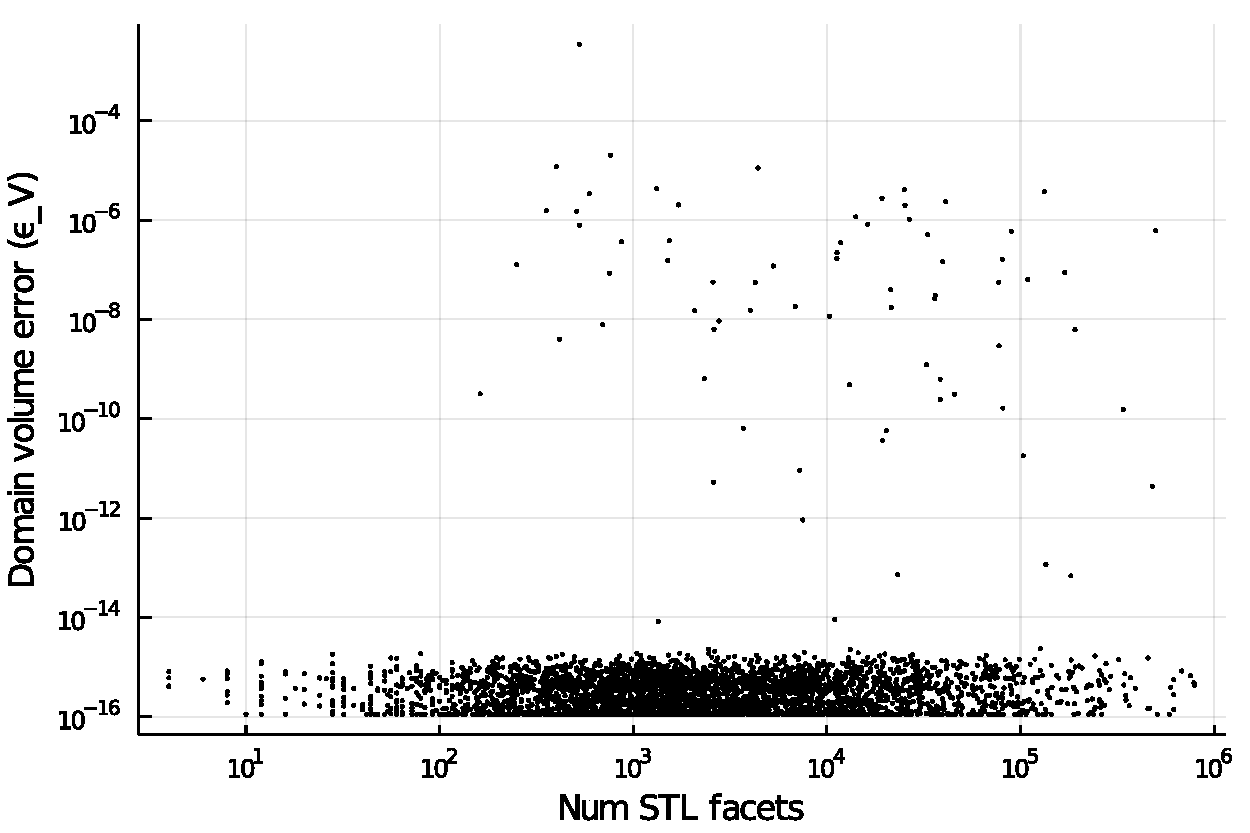
\includegraphics[width=0.95\textwidth]{../analysis/plots/num_stl_facets_volume_error}
\end{frame}

\begin{frame}{Thingi 10k dataset}
  \framesubtitle{Removing small facets}
  % a frequency graph may be better
  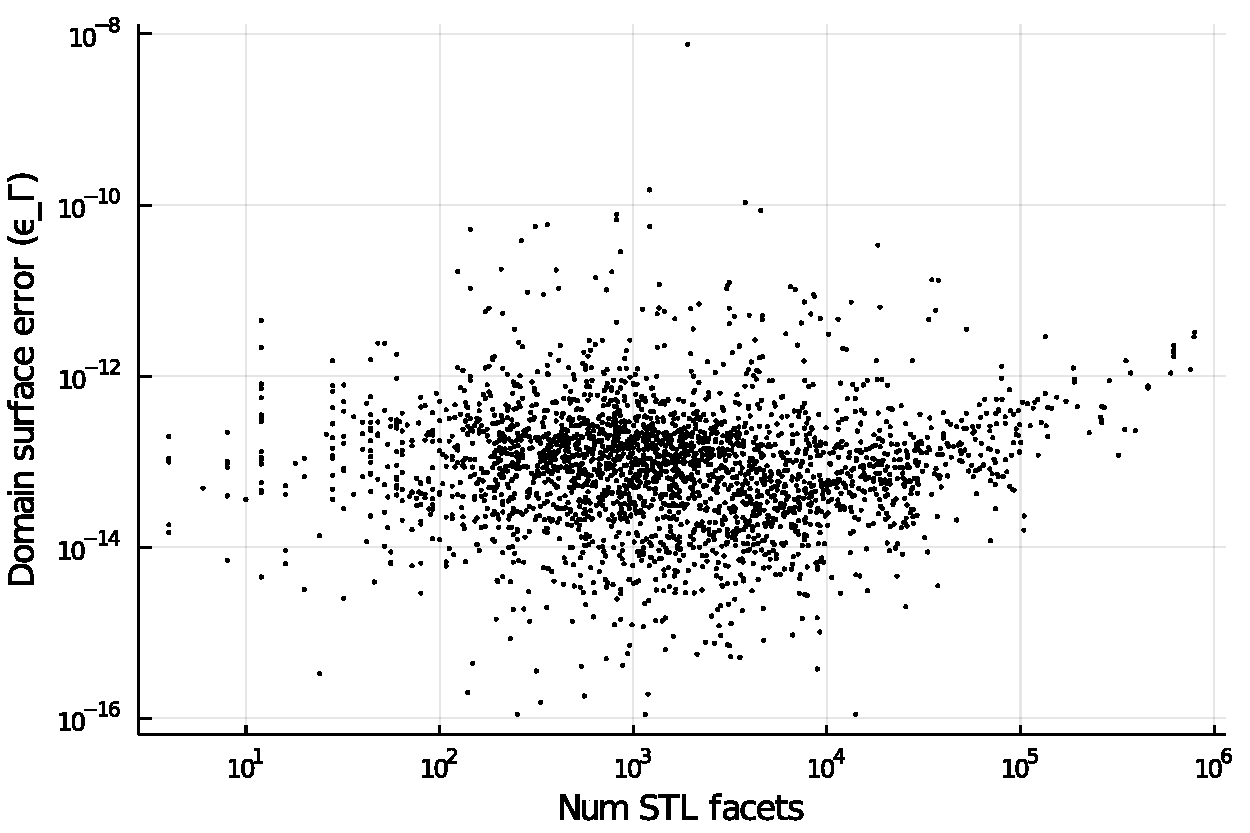
\includegraphics[width=0.95\textwidth]{../analysis/plots/num_stl_facets_surface_error}
\end{frame}

\begin{frame}{Robustness matrix}
  \framesubtitle{Summary}

  \textbf{100\%} of ended test have volume and surface error bounded 
  ($\epsilon_{vol} < 10^{-14}$,$\epsilon_{surf} < 10^{-12}$) 

  \begin{block}

  The mesh sizes have $n_{max}$ multiple of 14 as the bounding box is expanded 
  a factor $0.2$ in each direction, thus the domain is 1.4 times the 
  bounding box per axis. The background cells will match the STL bounding box, 
  stressing even more the algorithm.
  \end{block}

  \vfill{}
  NOTE: Due to large computational requirements (time/memory),
  some tests have not ended.
  Those points are missing at the lowest and largest sizes.
  \begin{itemize}
    \item
      Low $n_{max}$: large amount of STL facets per cell
    \item
      High $n_{max}$: large background mesh

  \end{itemize}
 

\end{frame}

\begin{frame}{Robustness matrix}
  \framesubtitle{Geometries}
  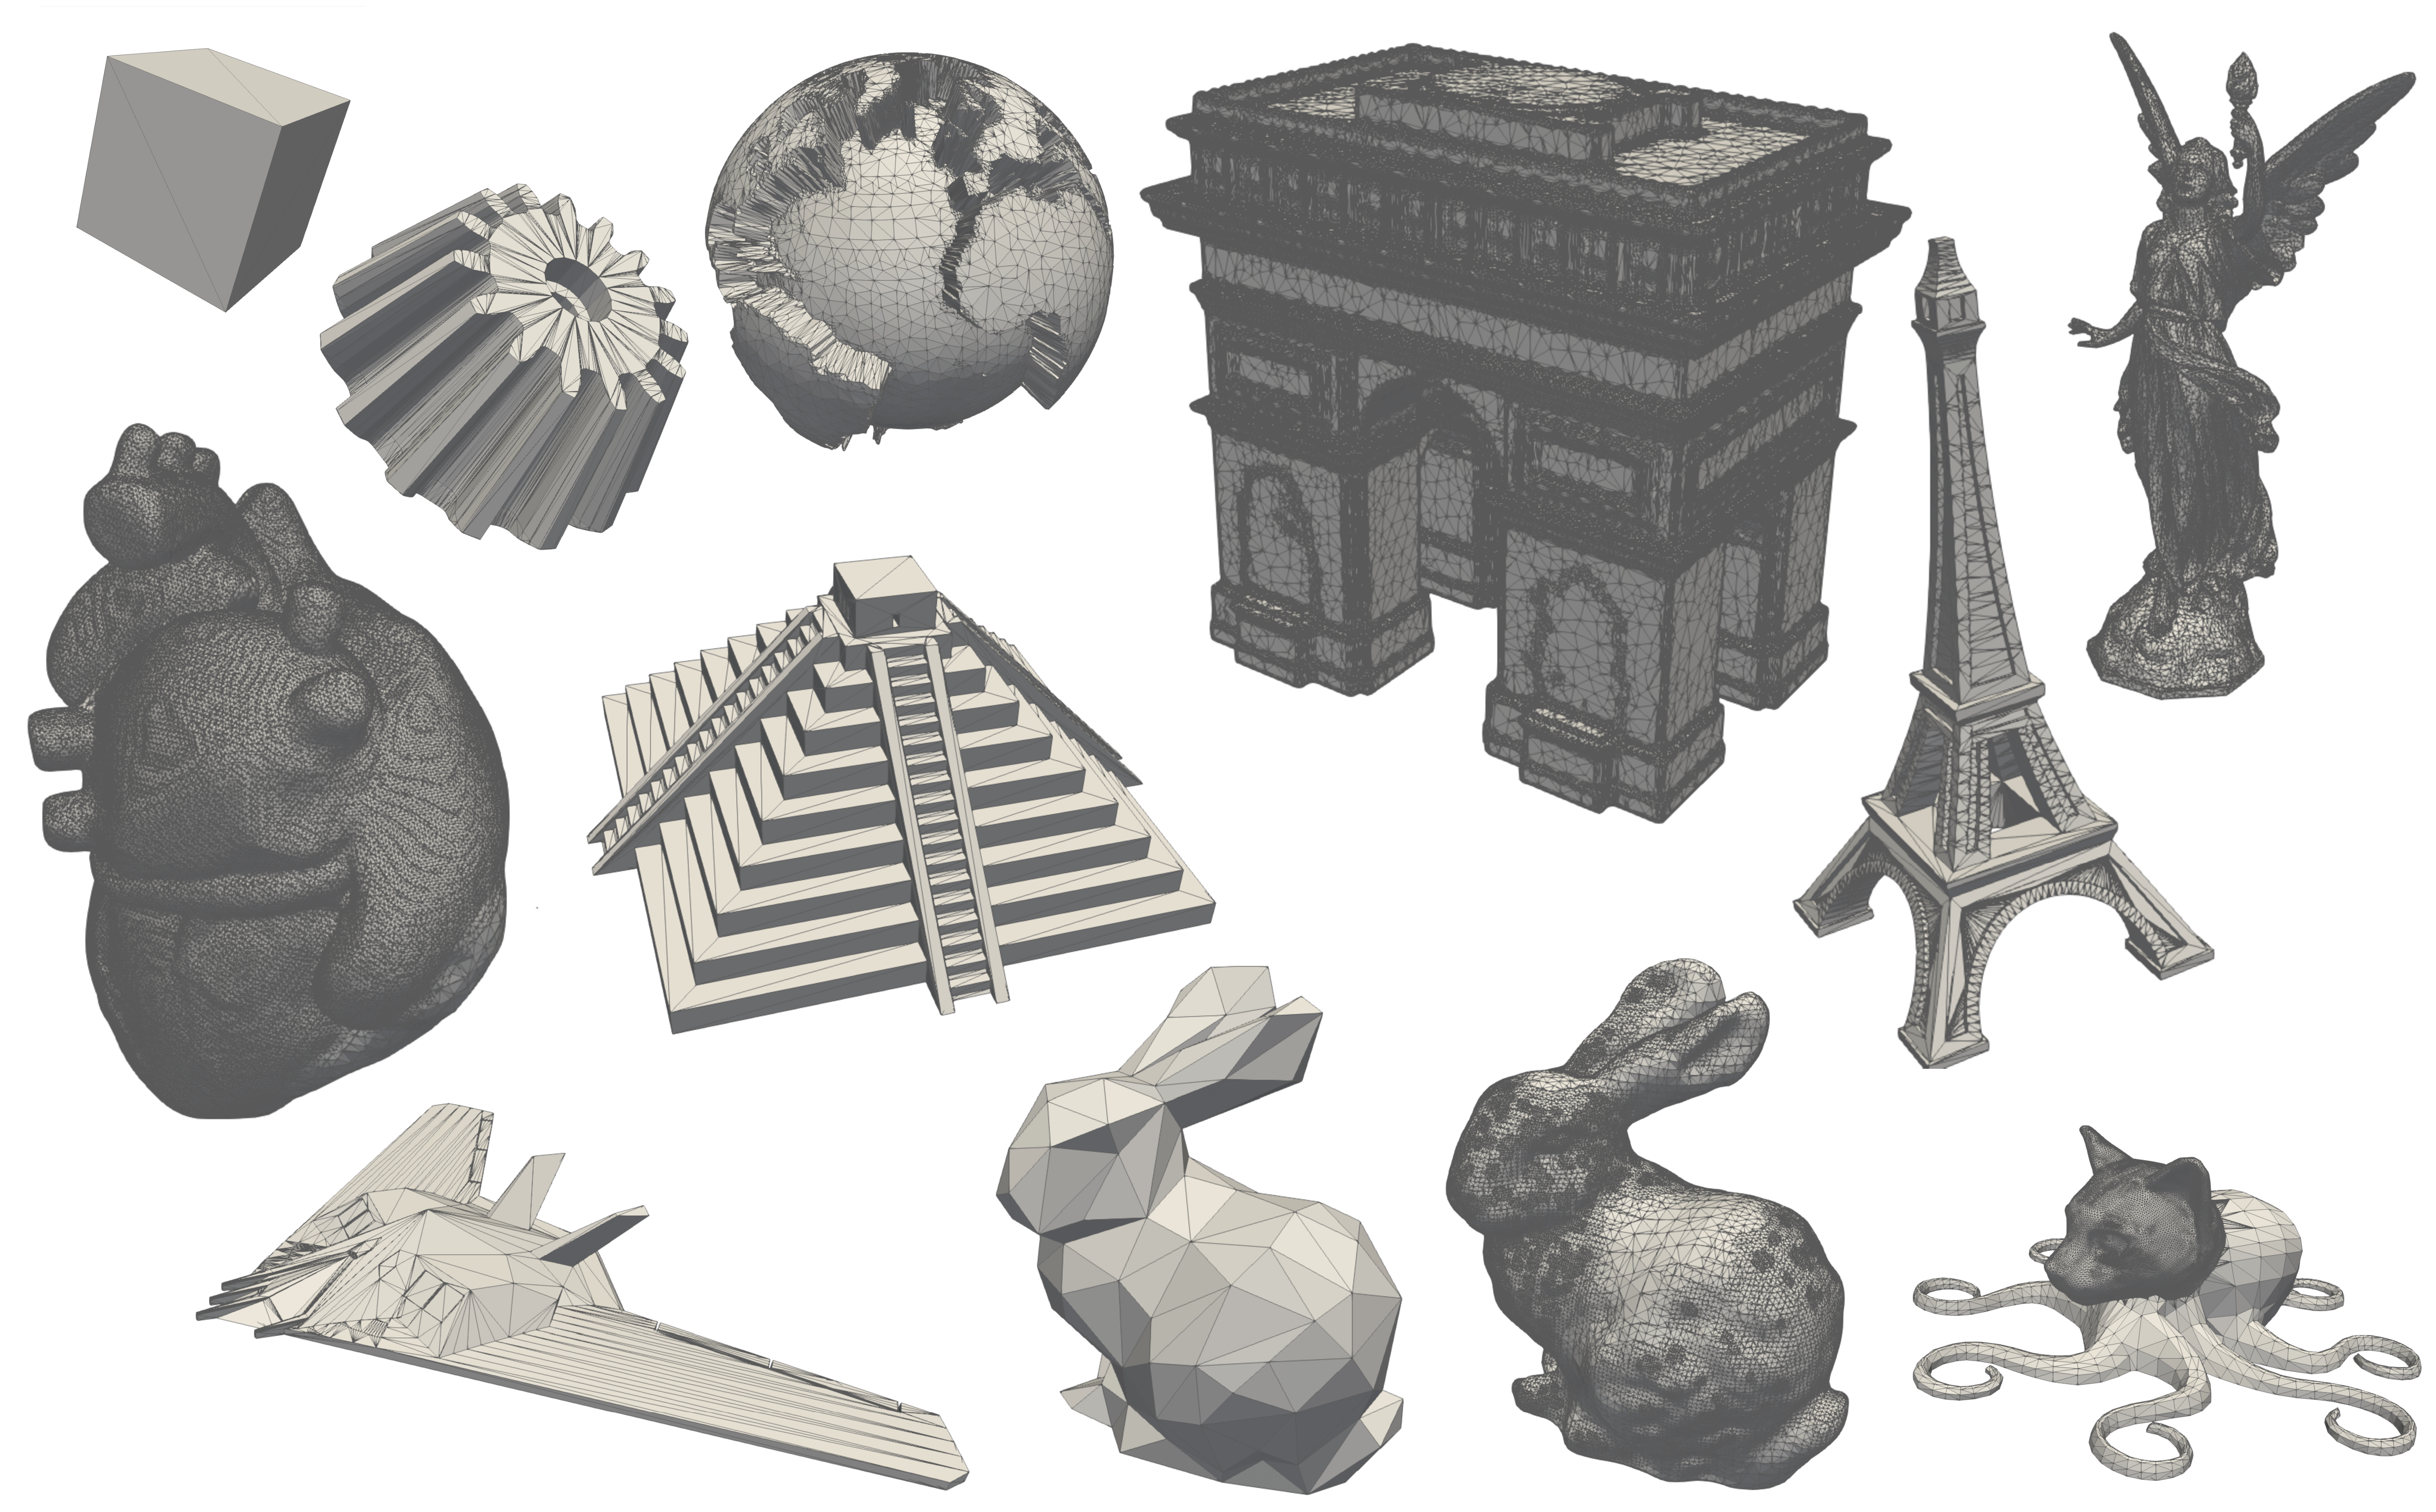
\includegraphics[width=0.95\textwidth]{matrix.pdf}
\end{frame}



\begin{frame}{Robustness matrix}
  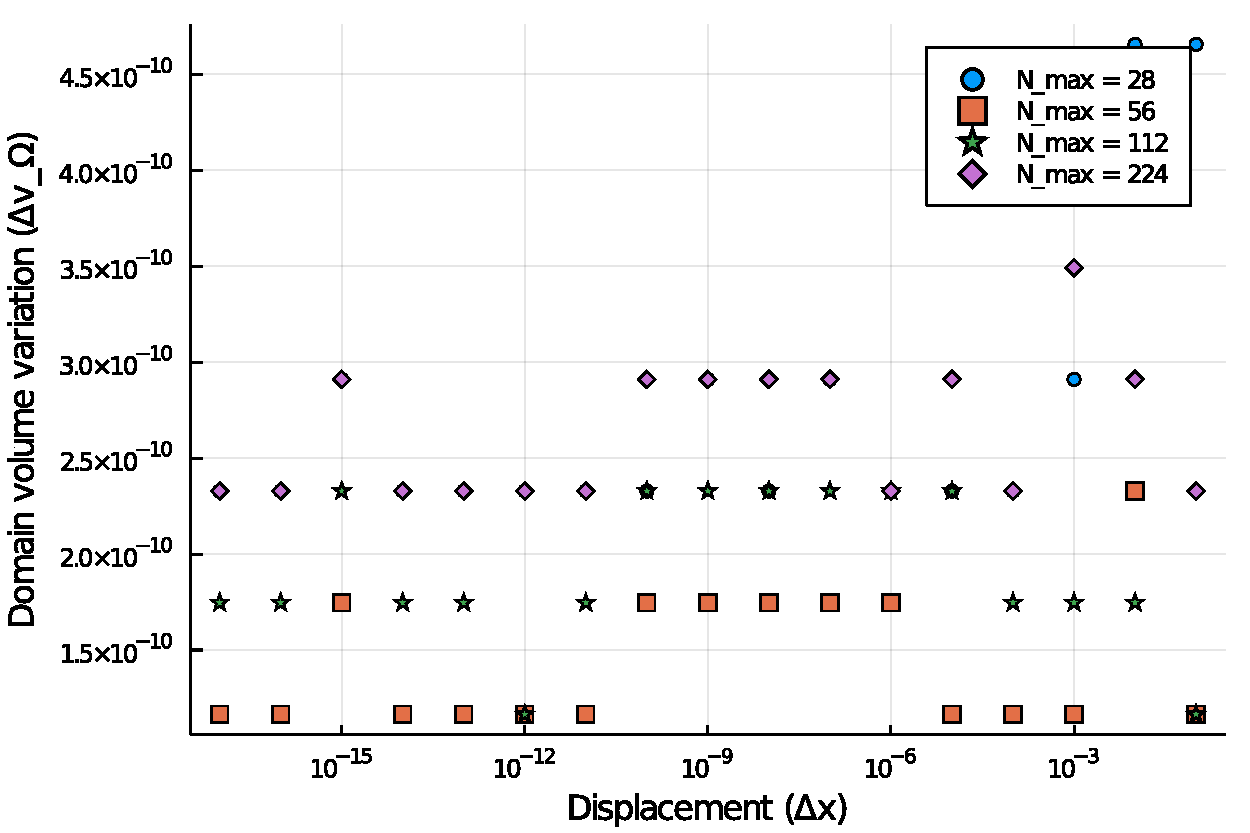
\includegraphics[width=0.95\textwidth]{../analysis/plots/name_441708_x_displacement_y_domain_volume.pdf}
  \put (-70,100) {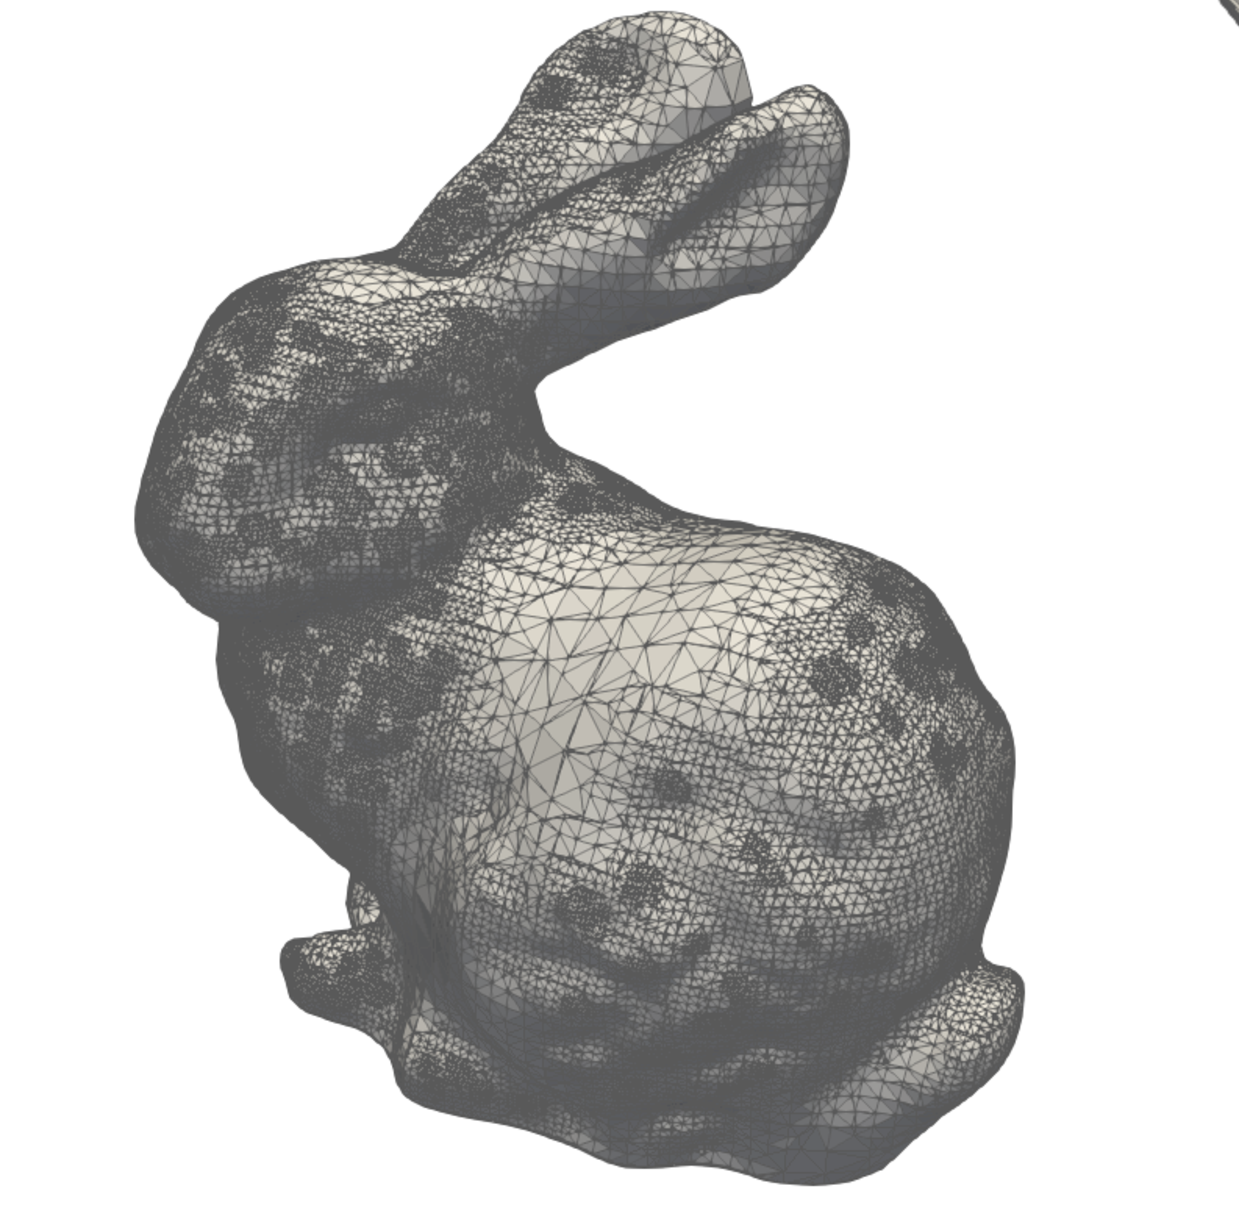
\includegraphics[width=0.2\textwidth]{441708}}
\end{frame}
\begin{frame}{Robustness matrix}
  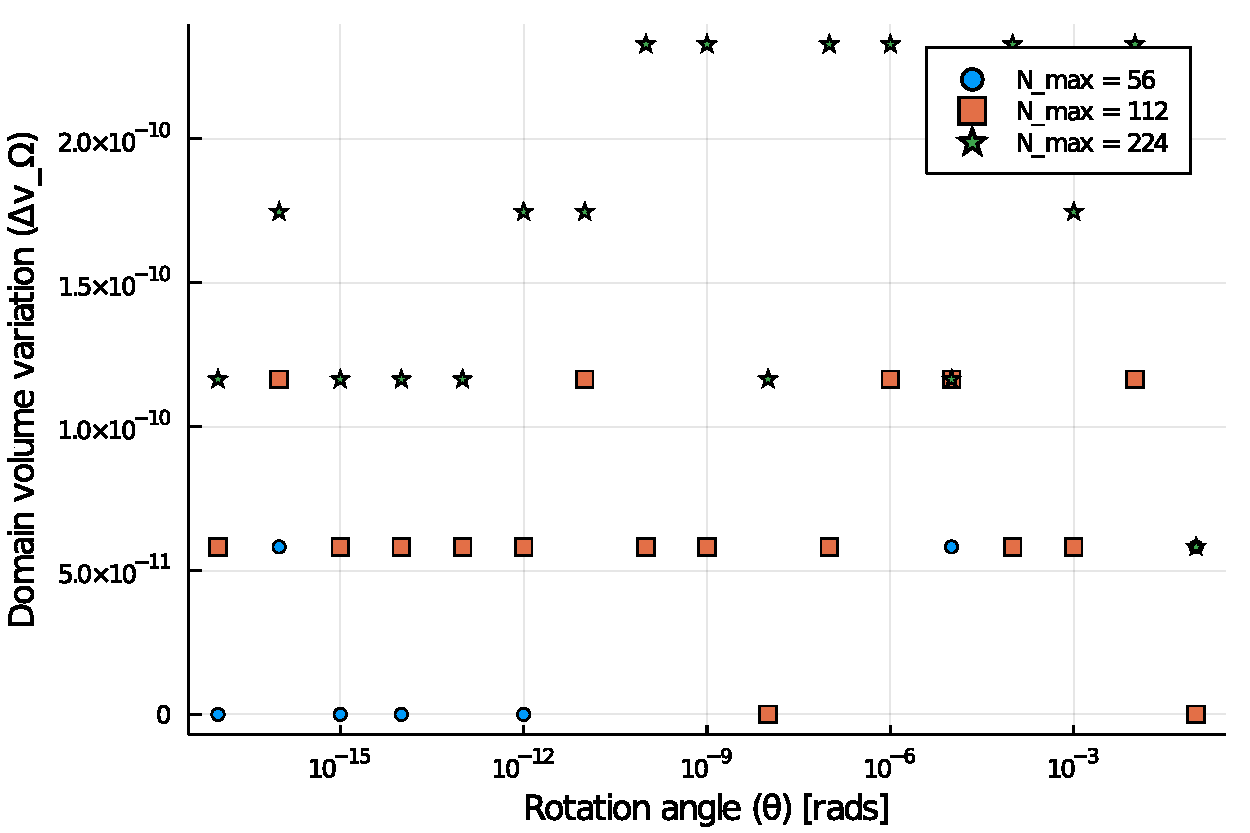
\includegraphics[width=0.95\textwidth]{../analysis/plots/name_441708_x_rotation_y_domain_volume.pdf}
  \put (-70,100) {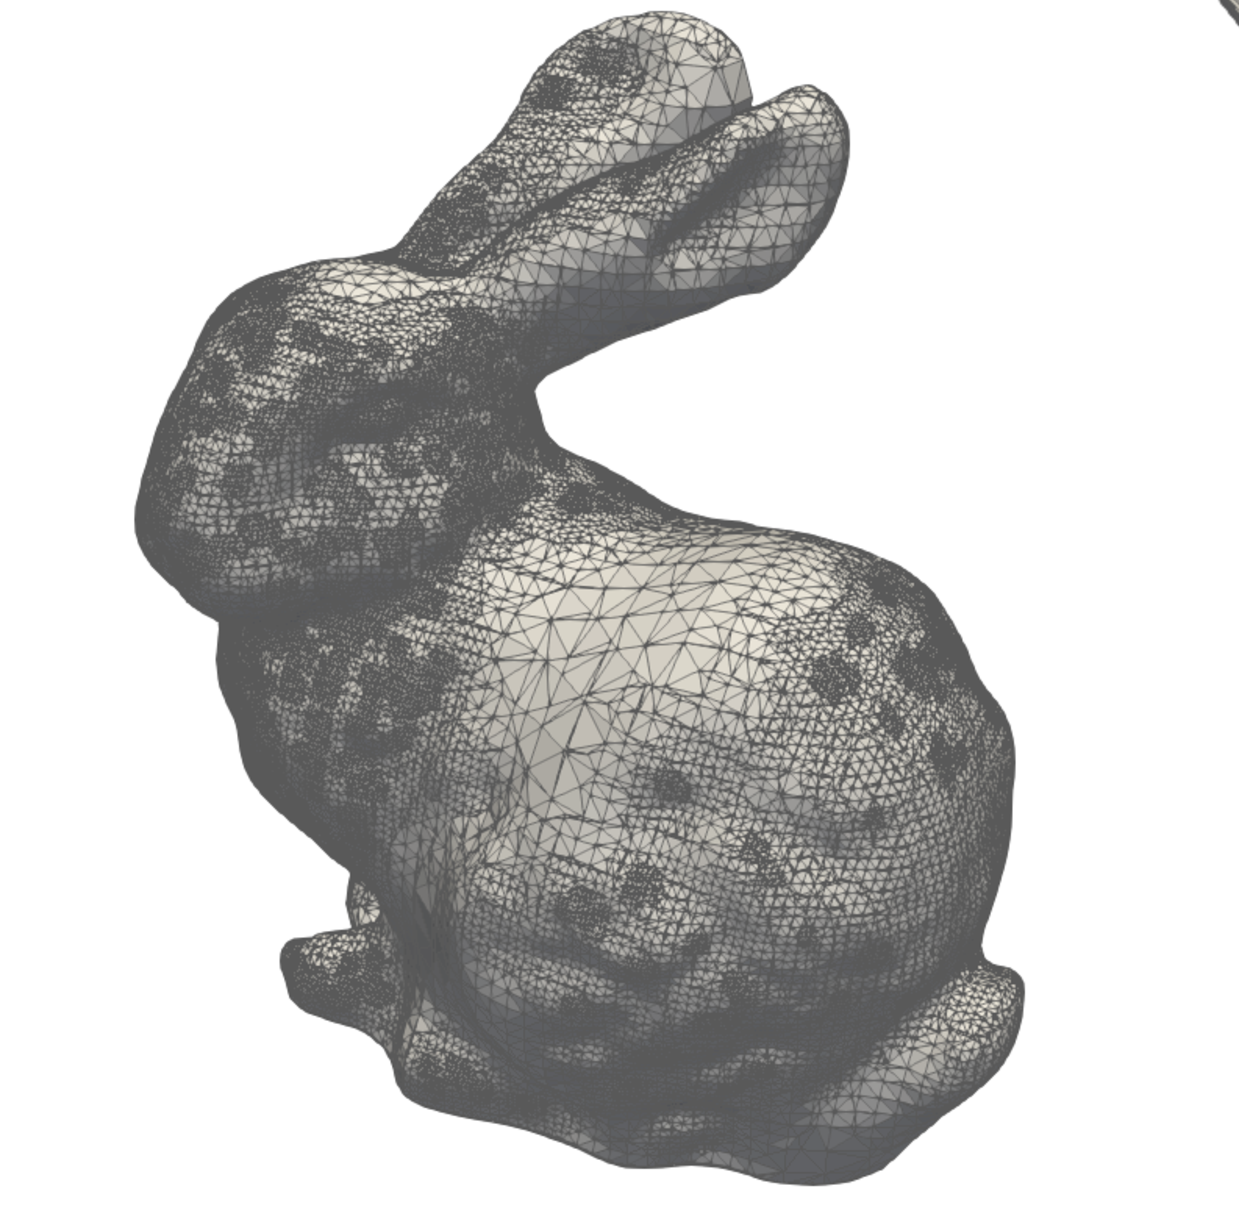
\includegraphics[width=0.2\textwidth]{441708}}
\end{frame}
\begin{frame}{Robustness matrix}
  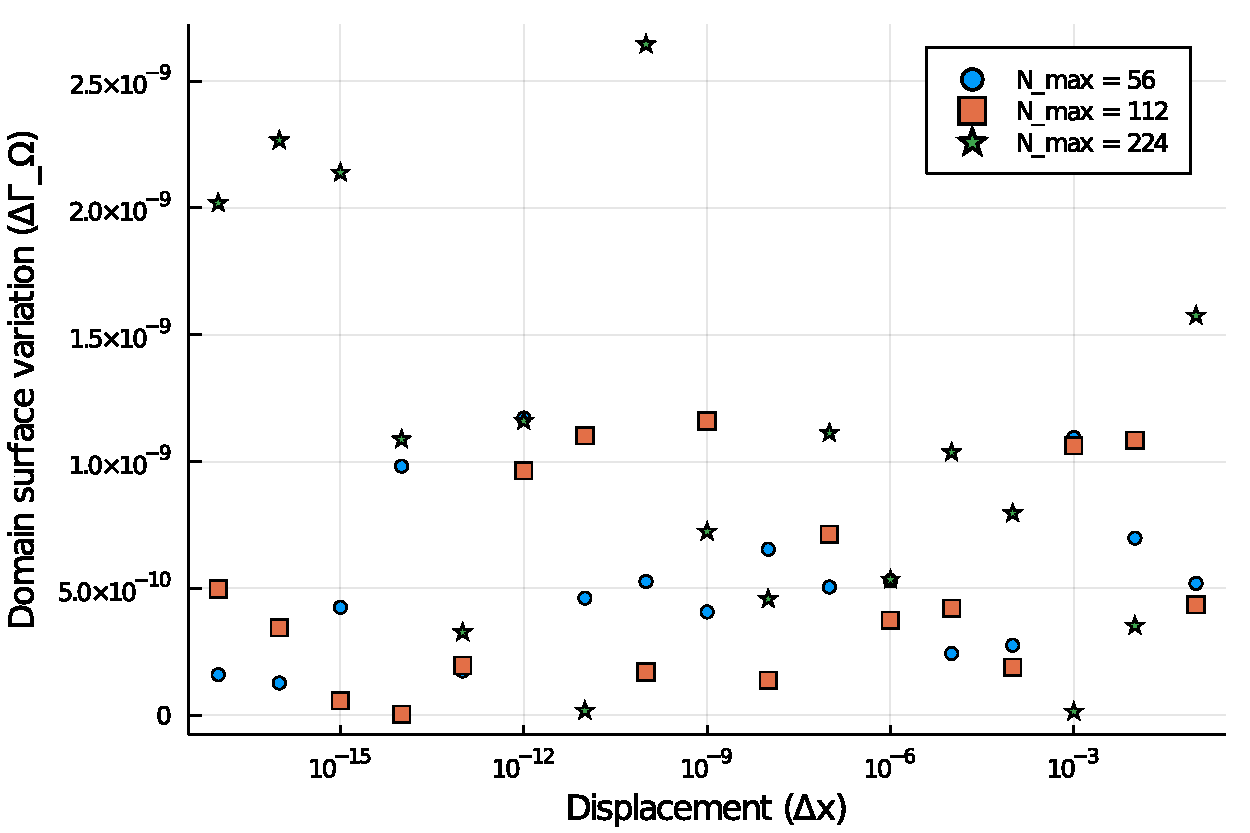
\includegraphics[width=0.95\textwidth]{../analysis/plots/name_441708_x_displacement_y_domain_surface.pdf}
  \put (-70,100) {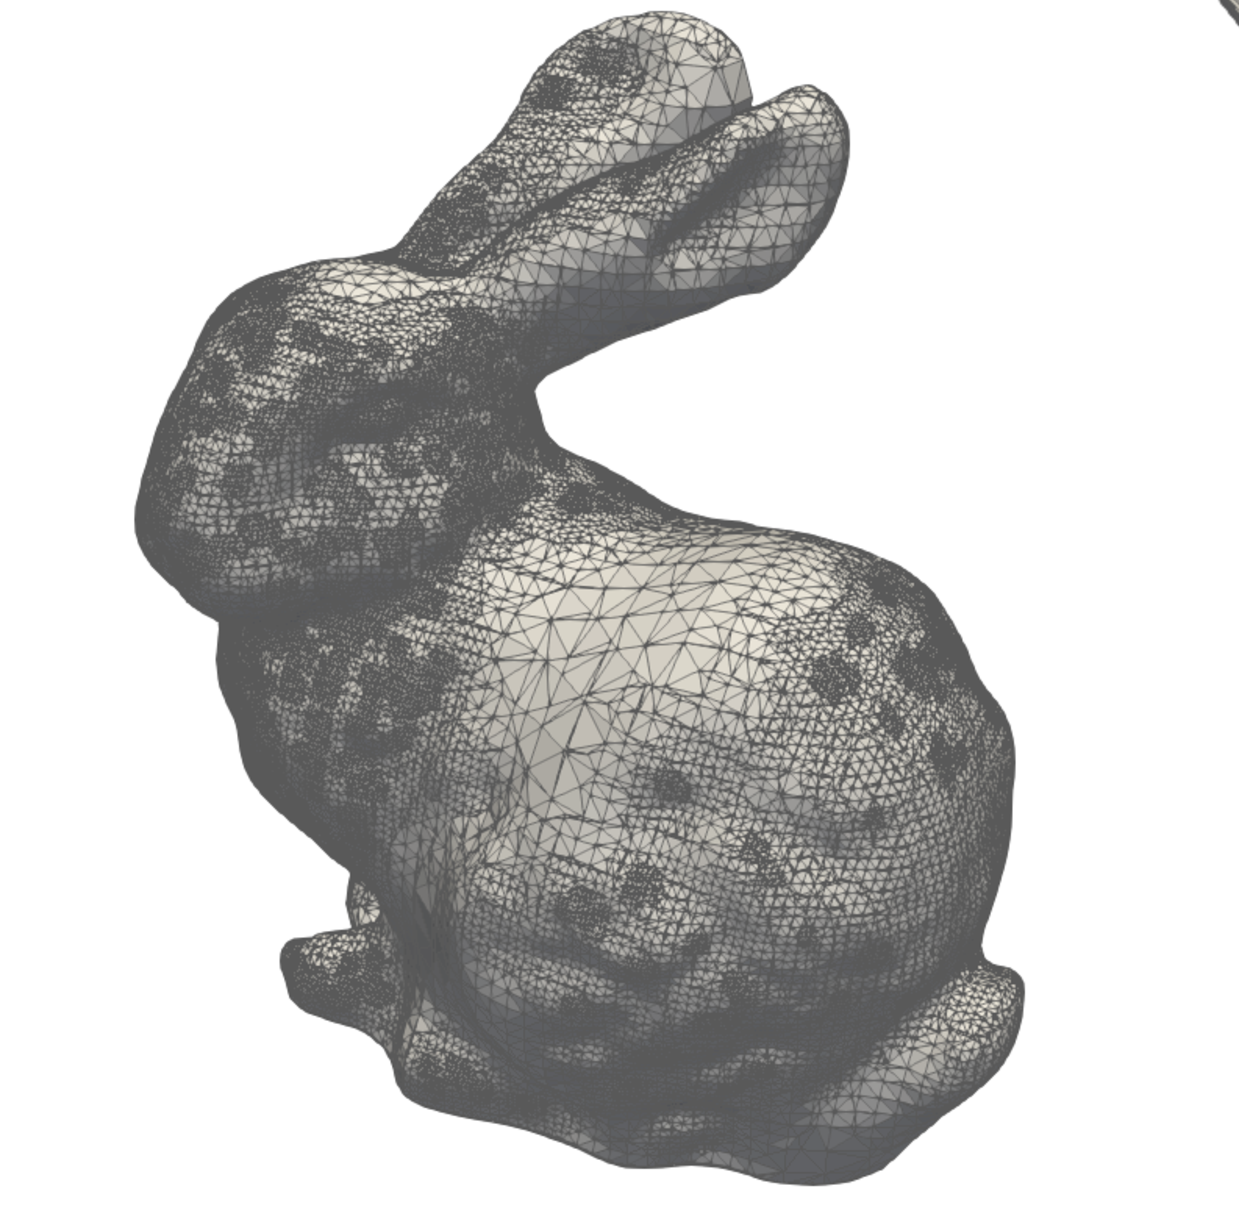
\includegraphics[width=0.2\textwidth]{441708}}
\end{frame}
\begin{frame}{Robustness matrix}
  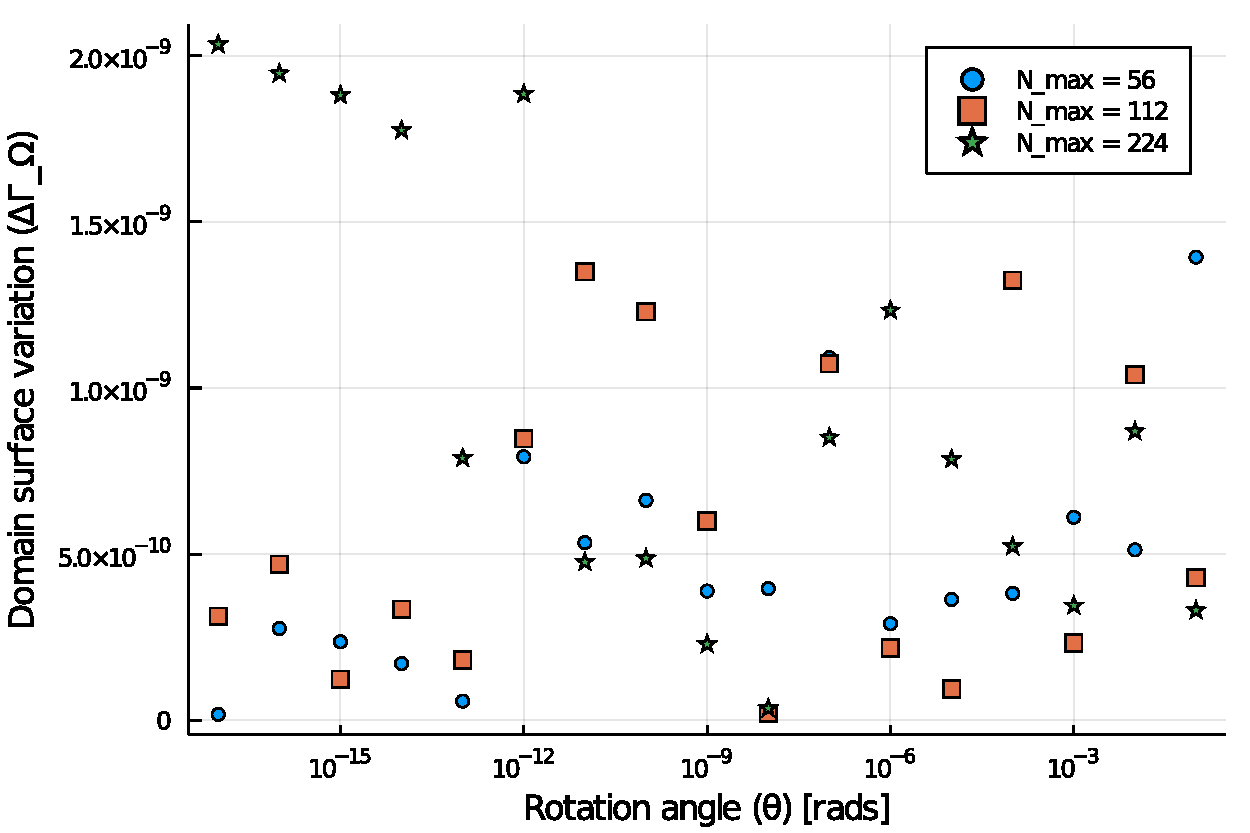
\includegraphics[width=0.95\textwidth]{../analysis/plots/name_441708_x_rotation_y_domain_surface.pdf}
  \put (-70,100) {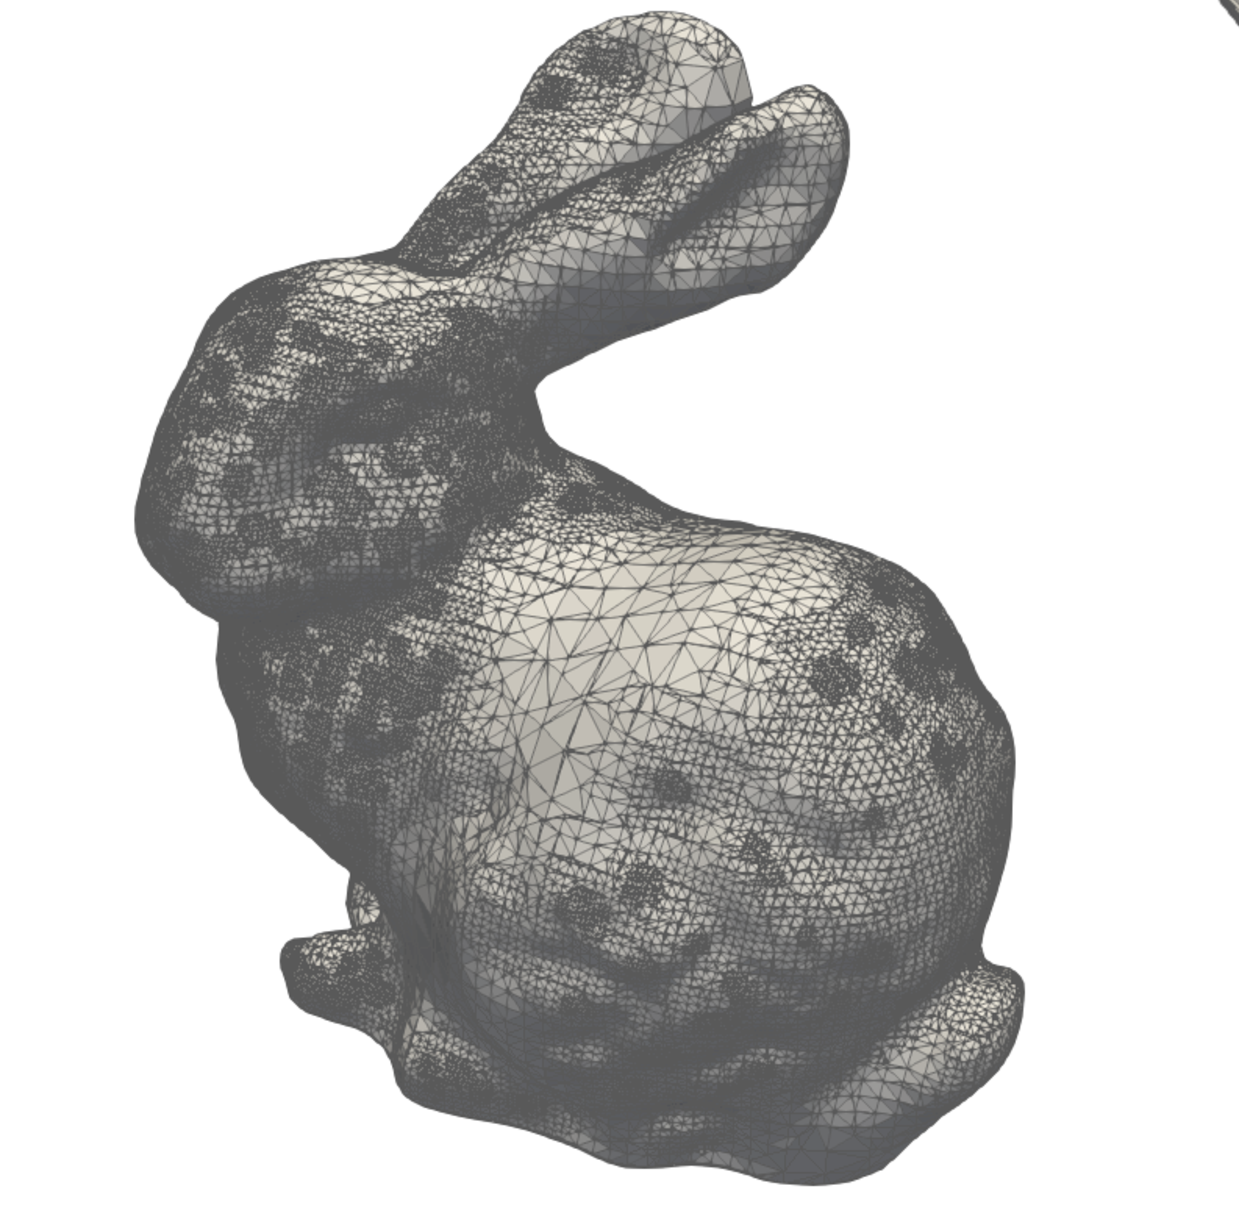
\includegraphics[width=0.2\textwidth]{441708}}
\end{frame}
\begin{frame}{Robustness matrix}
  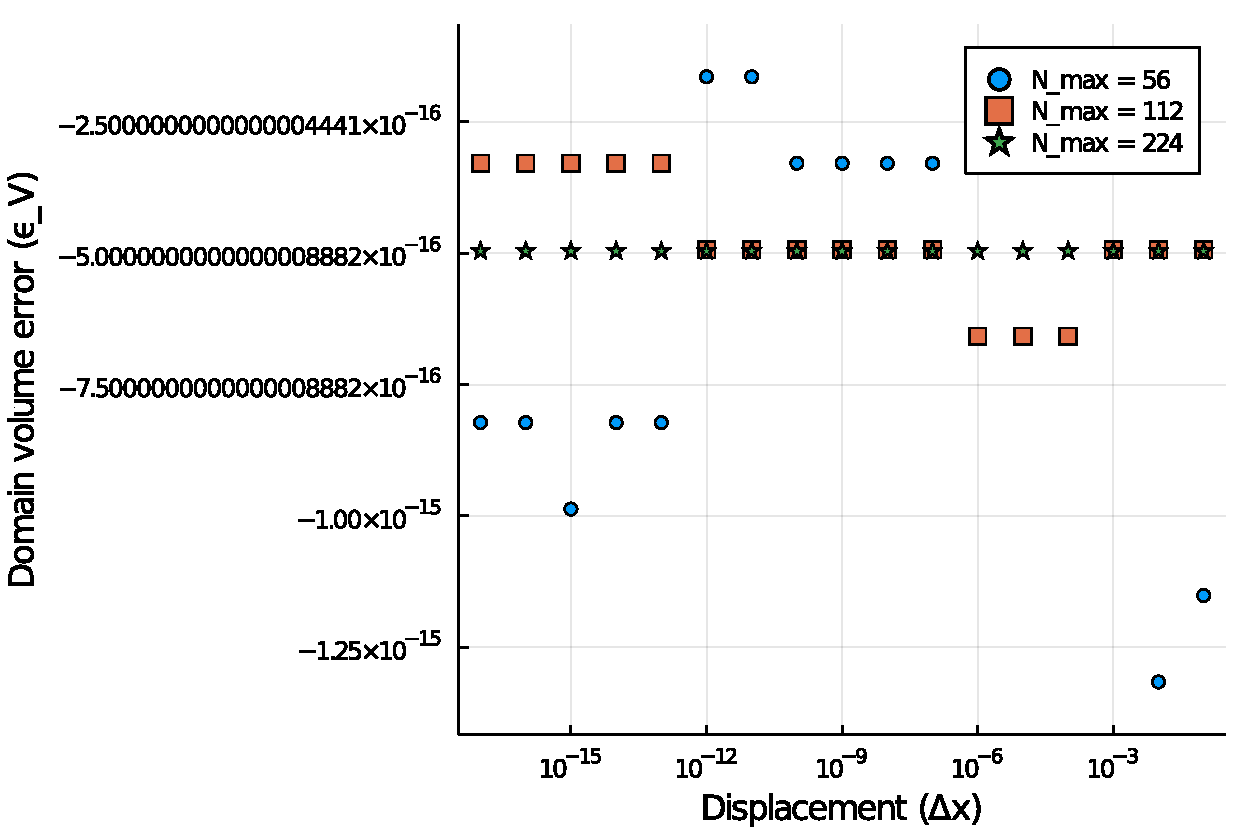
\includegraphics[width=0.95\textwidth]{../analysis/plots/name_441708_x_displacement_y_volume_error.pdf}
  \put (-70,100) {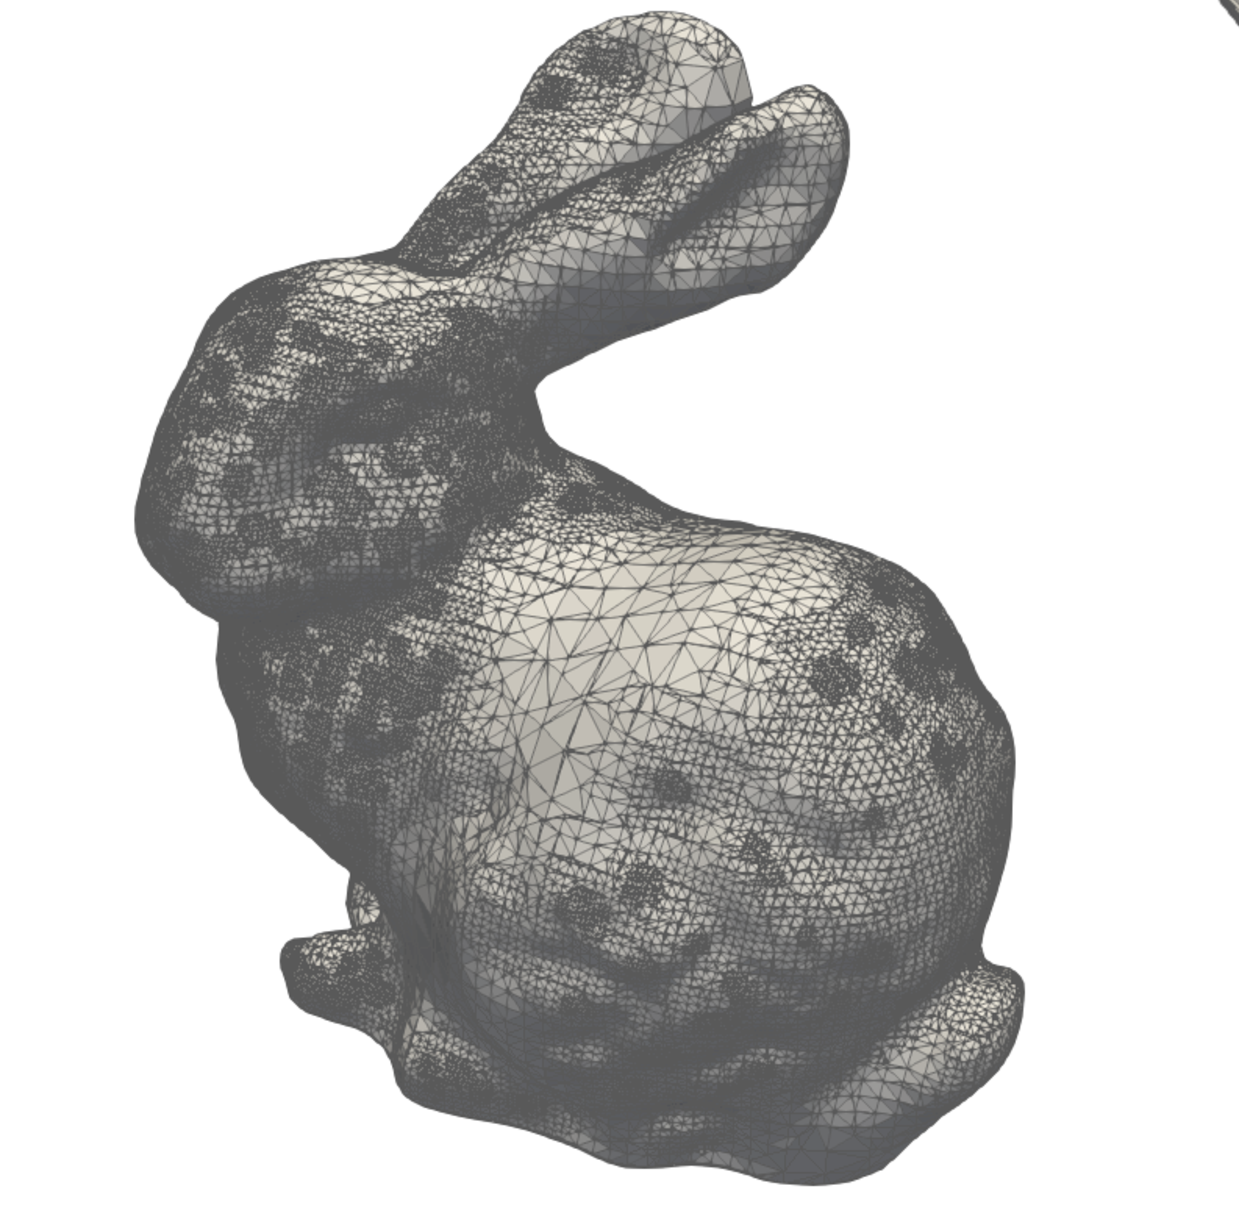
\includegraphics[width=0.2\textwidth]{441708}}
\end{frame}
\begin{frame}{Robustness matrix}
  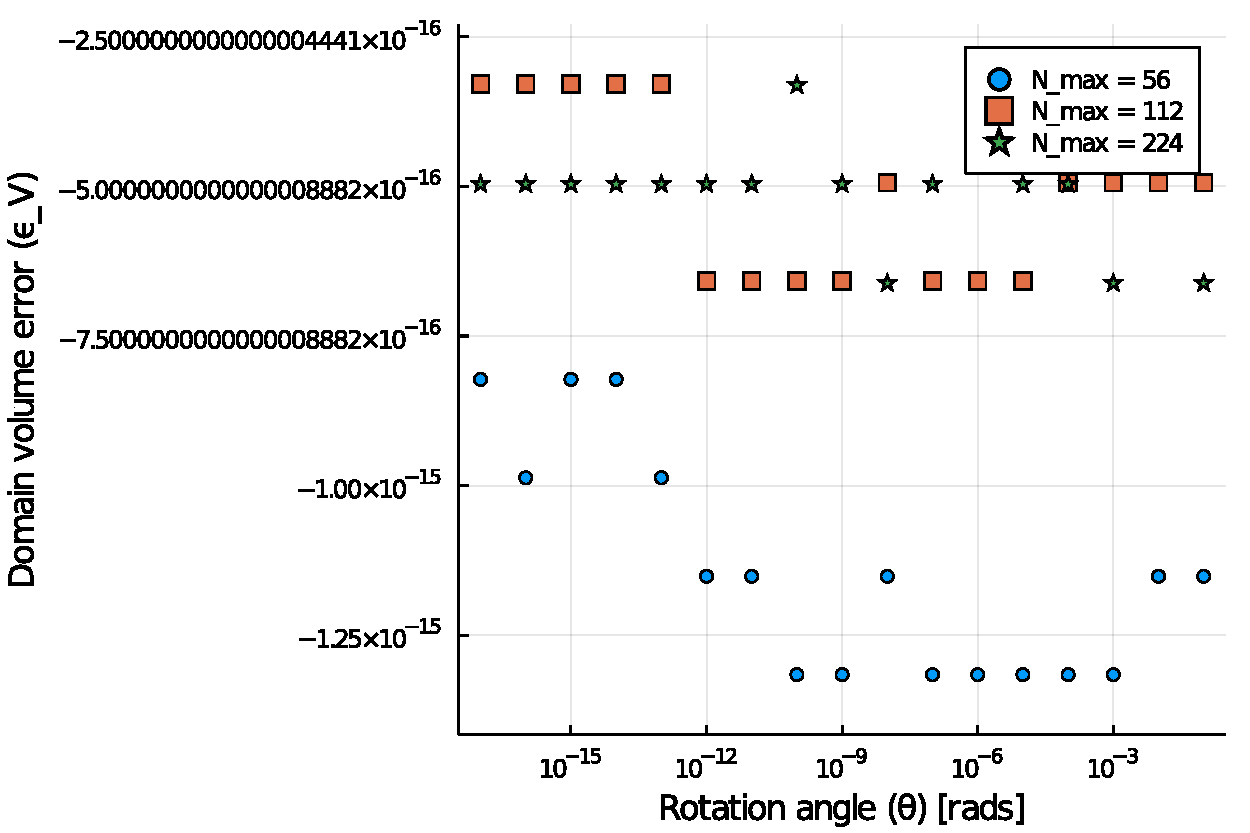
\includegraphics[width=0.95\textwidth]{../analysis/plots/name_441708_x_rotation_y_volume_error.pdf}
  \put (-70,100) {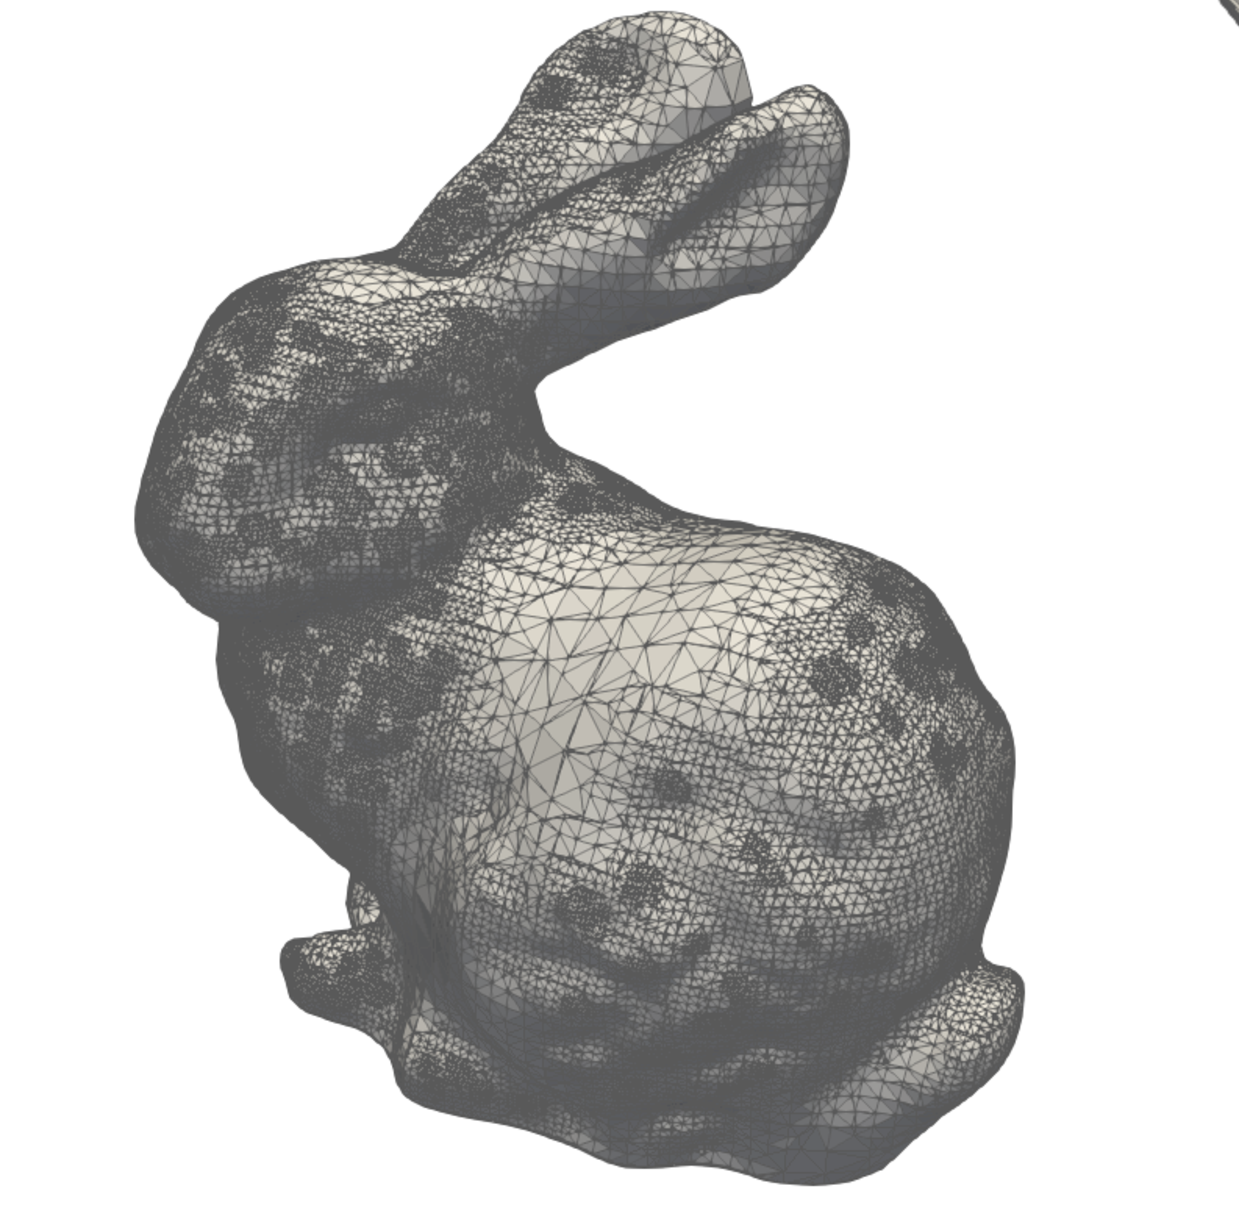
\includegraphics[width=0.2\textwidth]{441708}}
\end{frame}
\begin{frame}{Robustness matrix}
  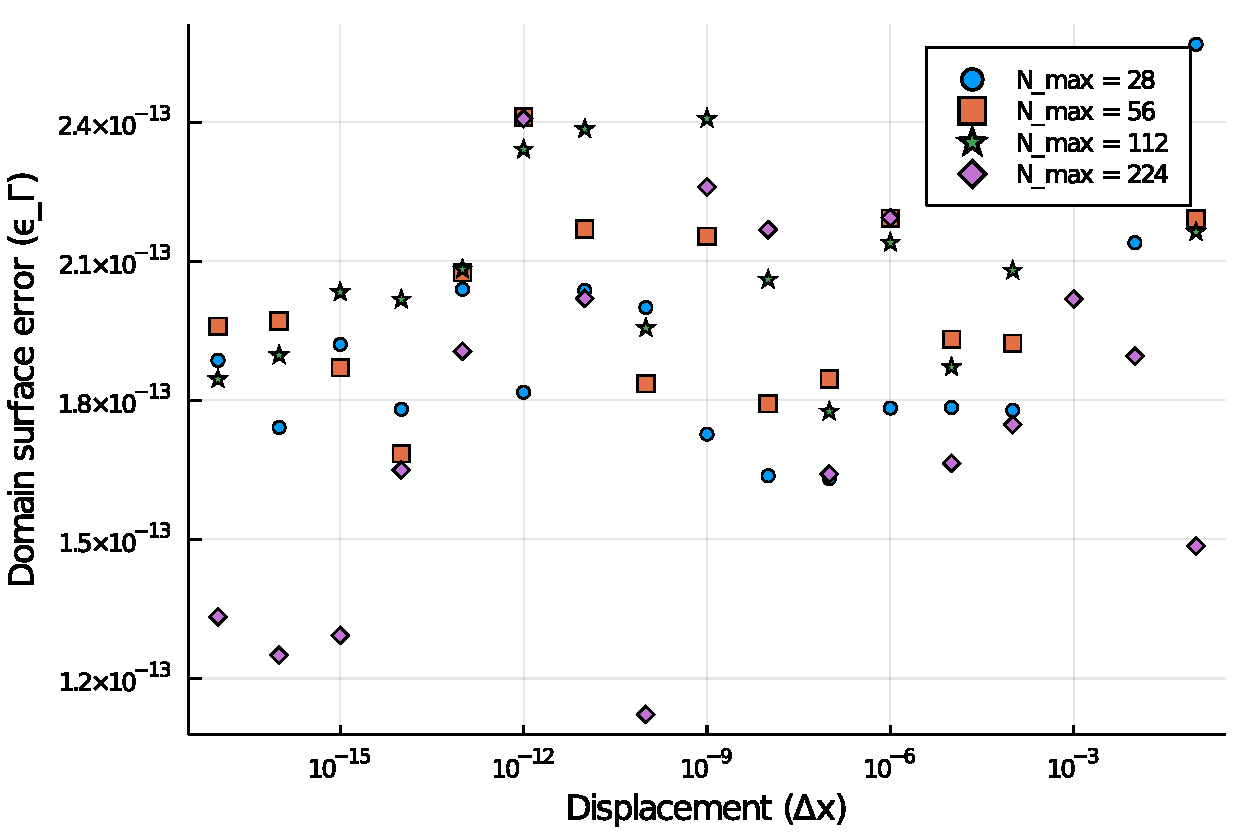
\includegraphics[width=0.95\textwidth]{../analysis/plots/name_441708_x_displacement_y_surface_error.pdf}
  \put (-70,100) {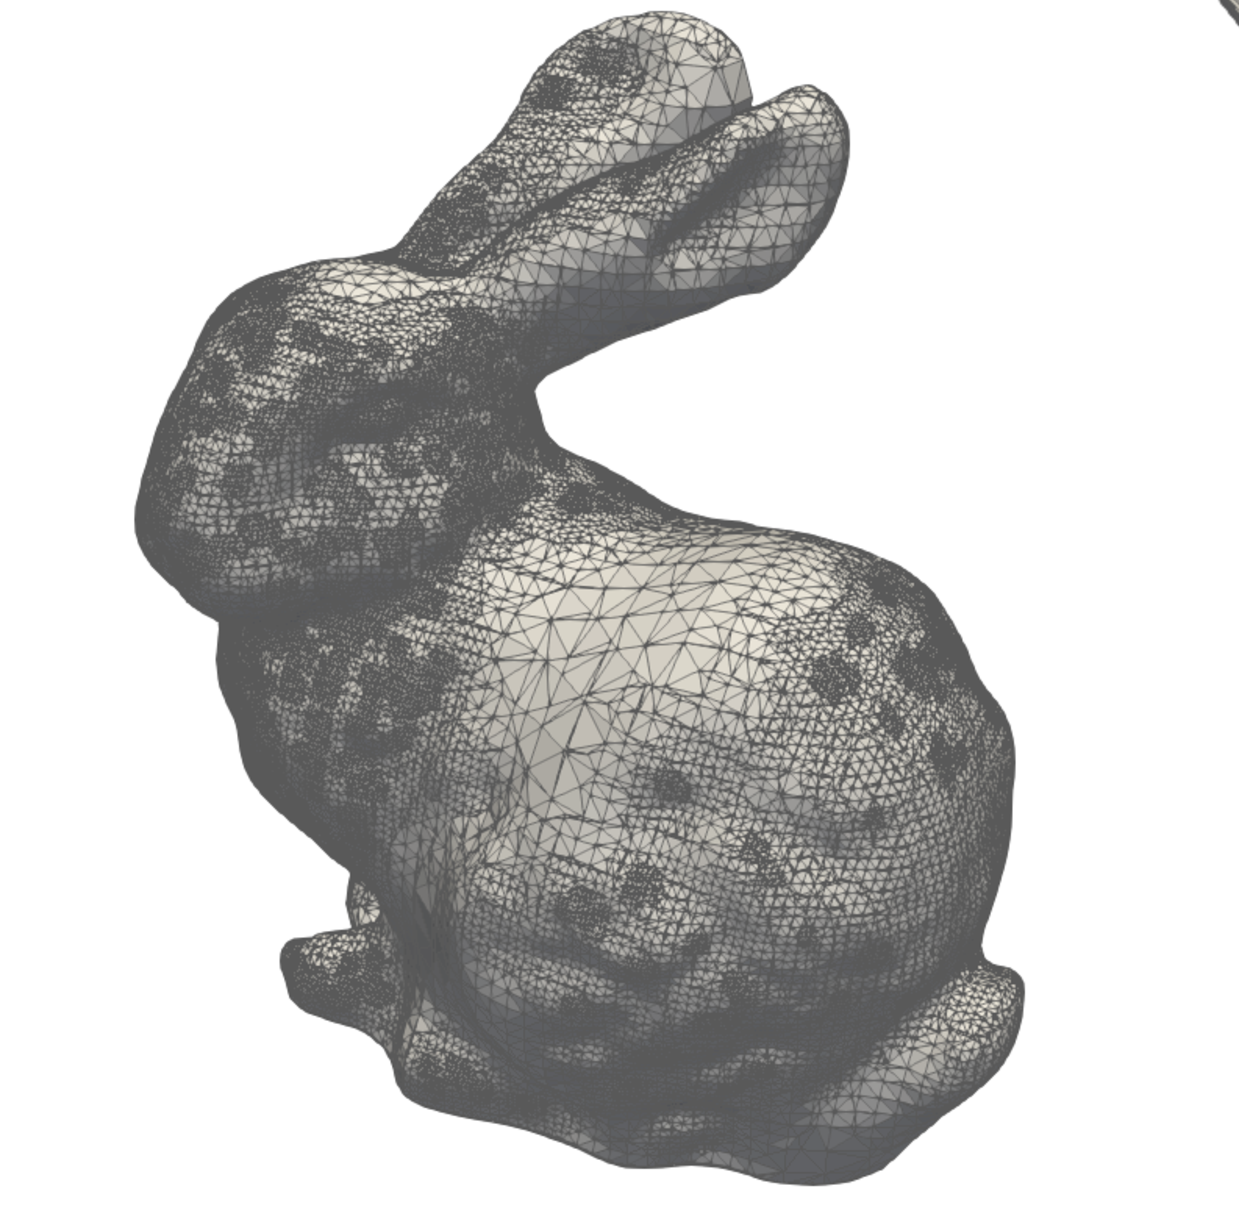
\includegraphics[width=0.2\textwidth]{441708}}
\end{frame}
\begin{frame}{Robustness matrix}
  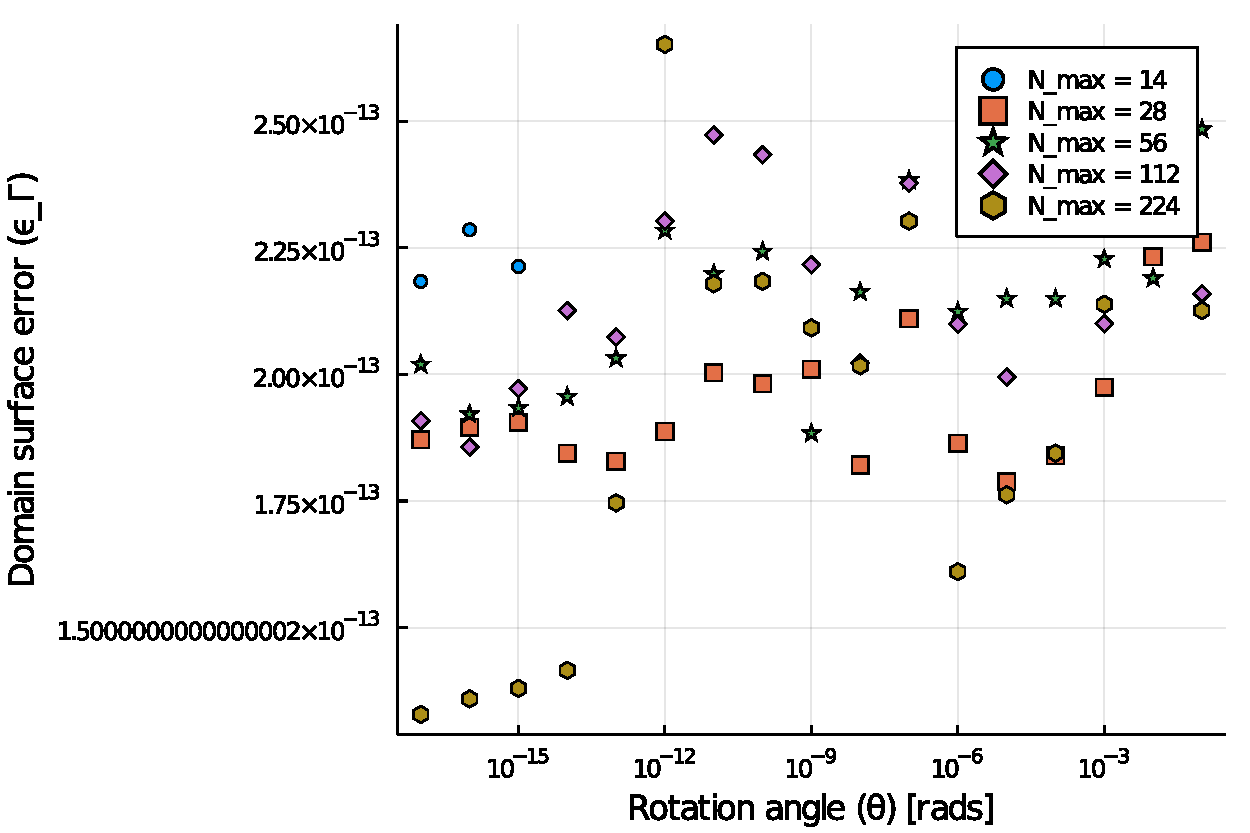
\includegraphics[width=0.95\textwidth]{../analysis/plots/name_441708_x_rotation_y_surface_error.pdf}
  \put (-70,100) {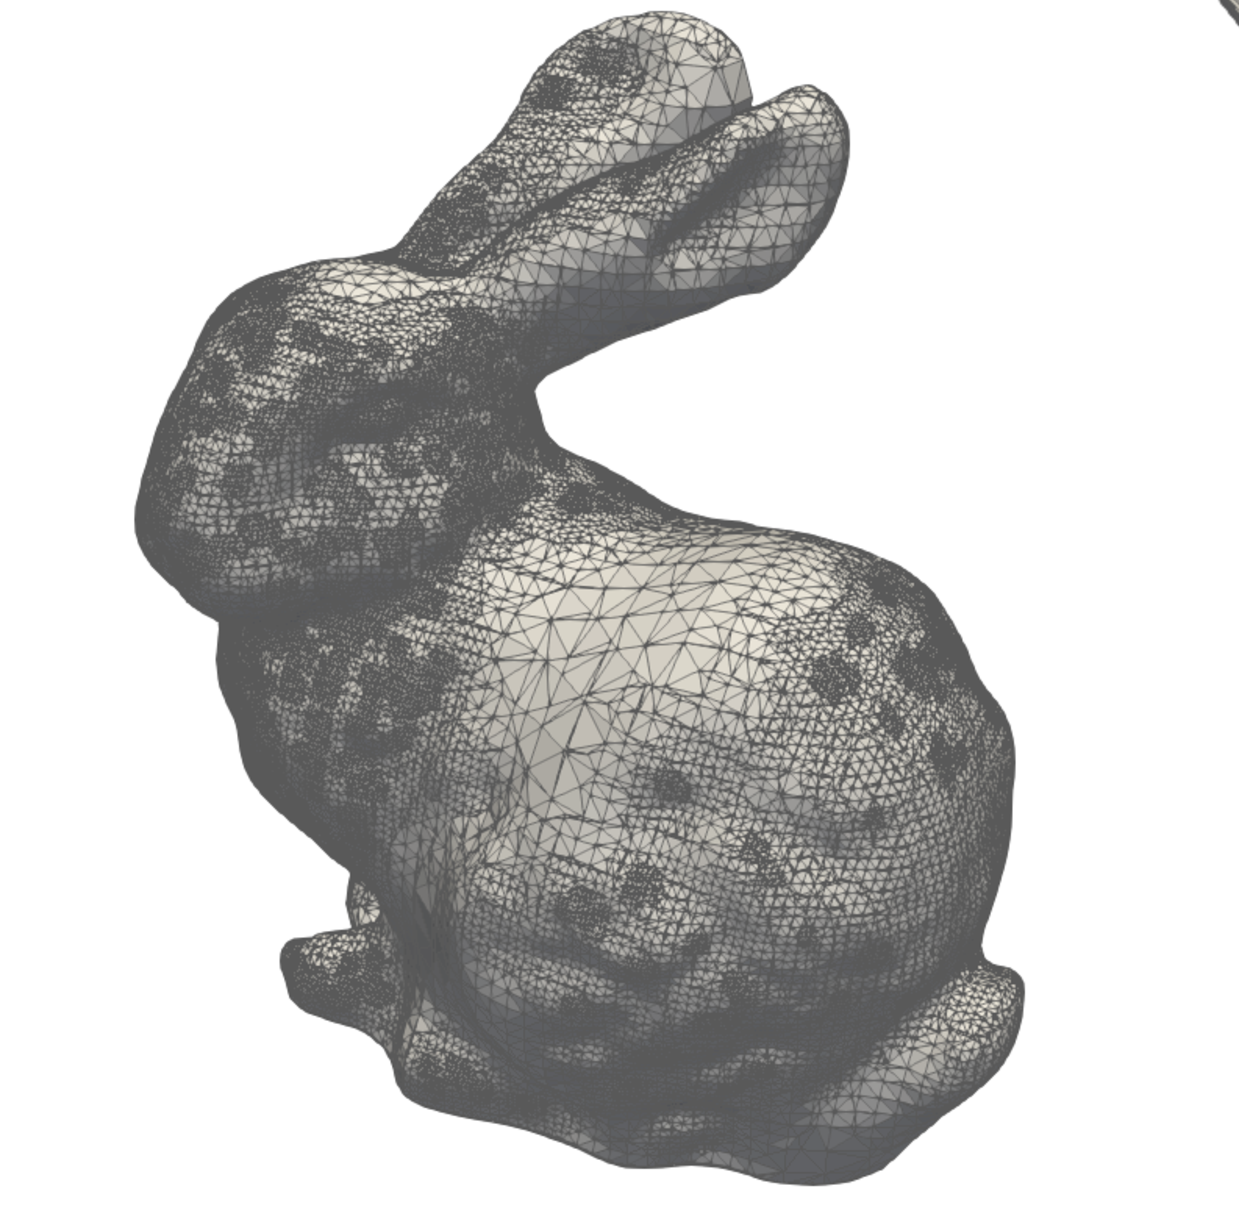
\includegraphics[width=0.2\textwidth]{441708}}
\end{frame}
\begin{frame}{Robustness matrix}
  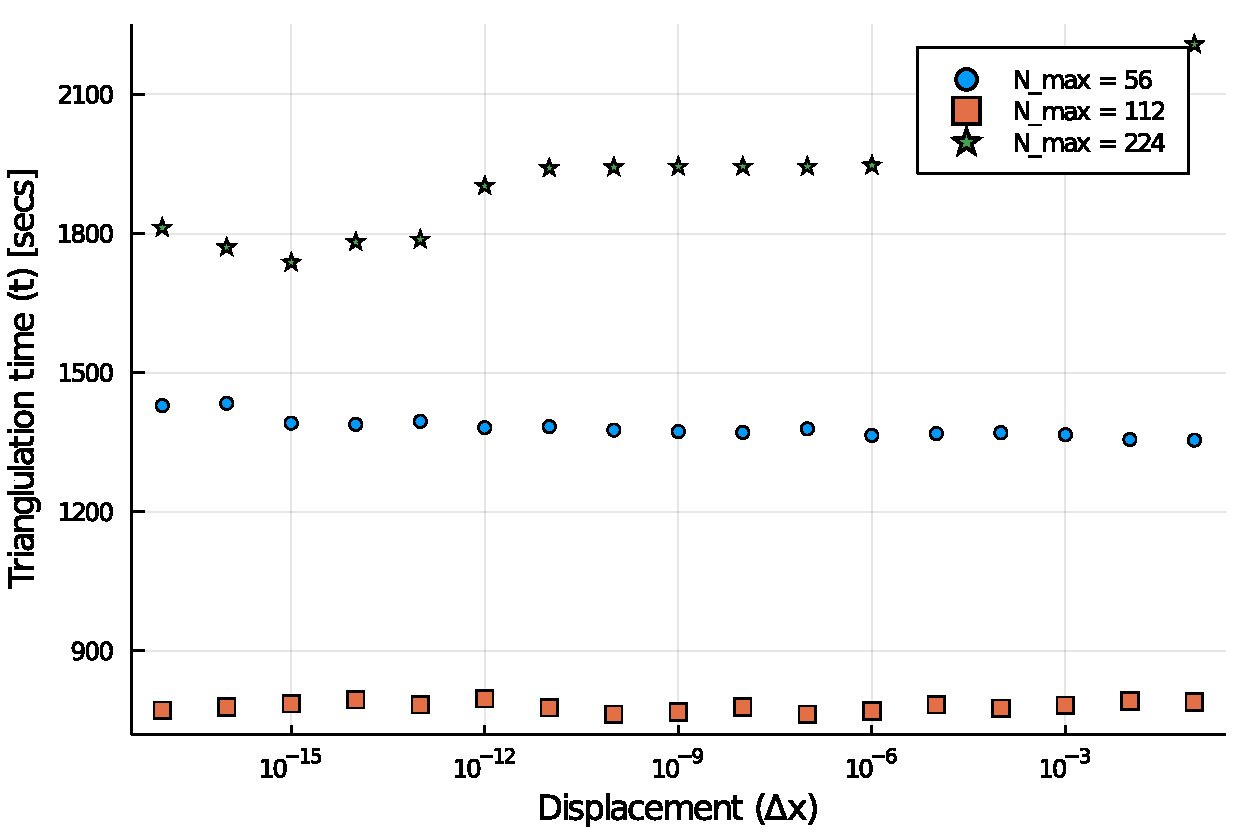
\includegraphics[width=0.95\textwidth]{../analysis/plots/name_441708_x_displacement_y_time.pdf}
  \put (-70,100) {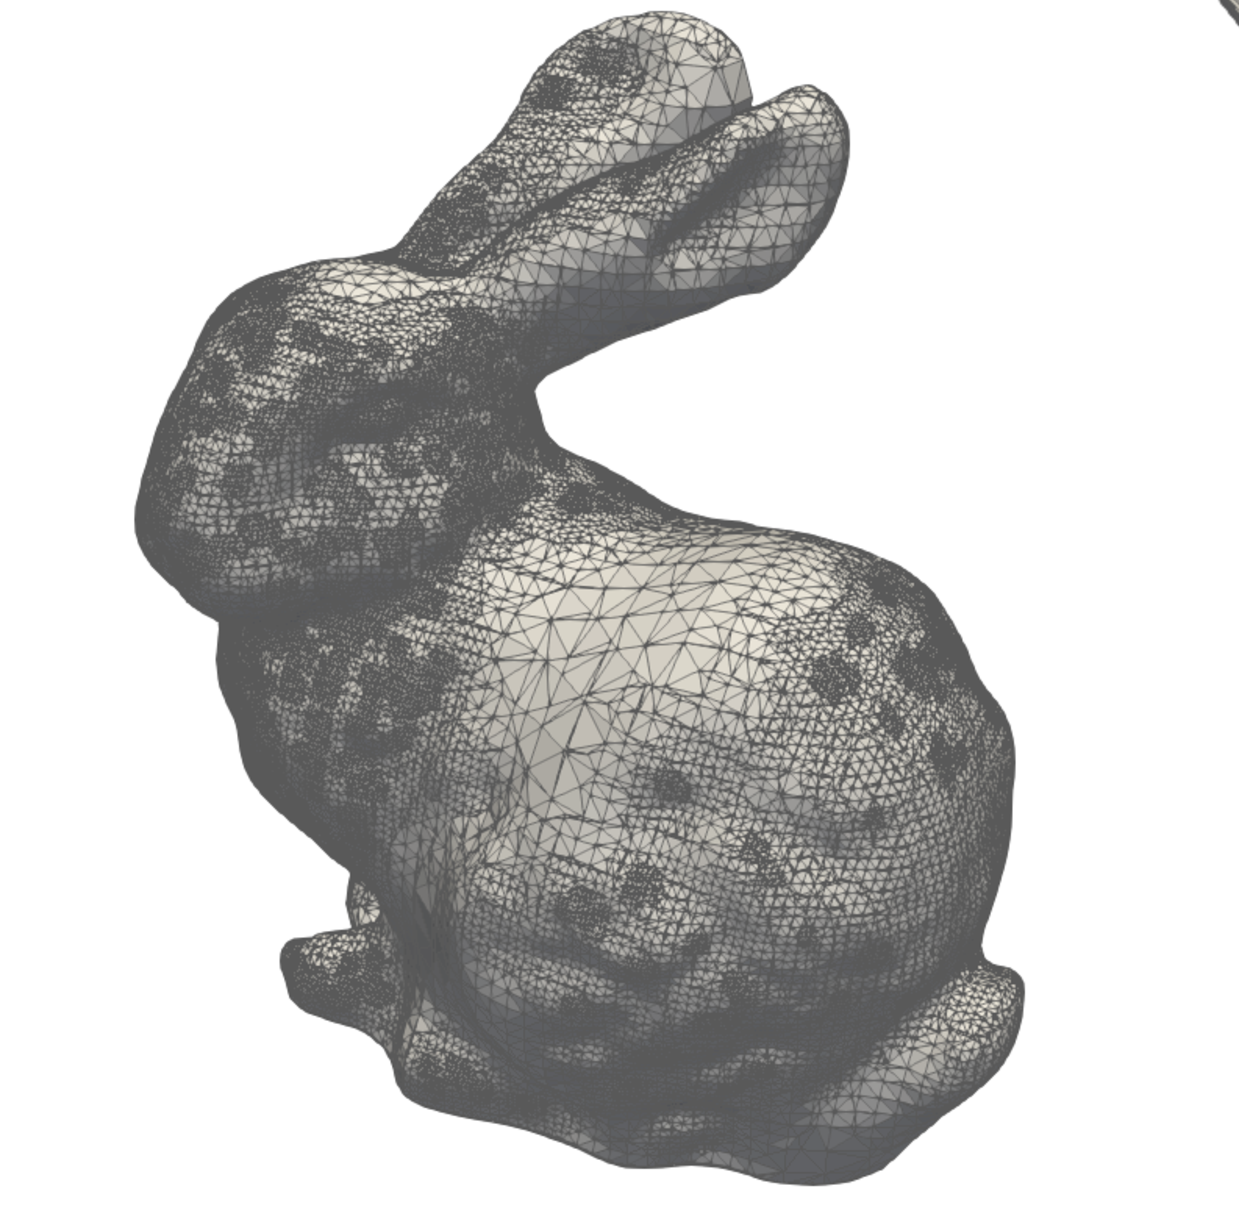
\includegraphics[width=0.2\textwidth]{441708}}
\end{frame}
\begin{frame}{Robustness matrix}
  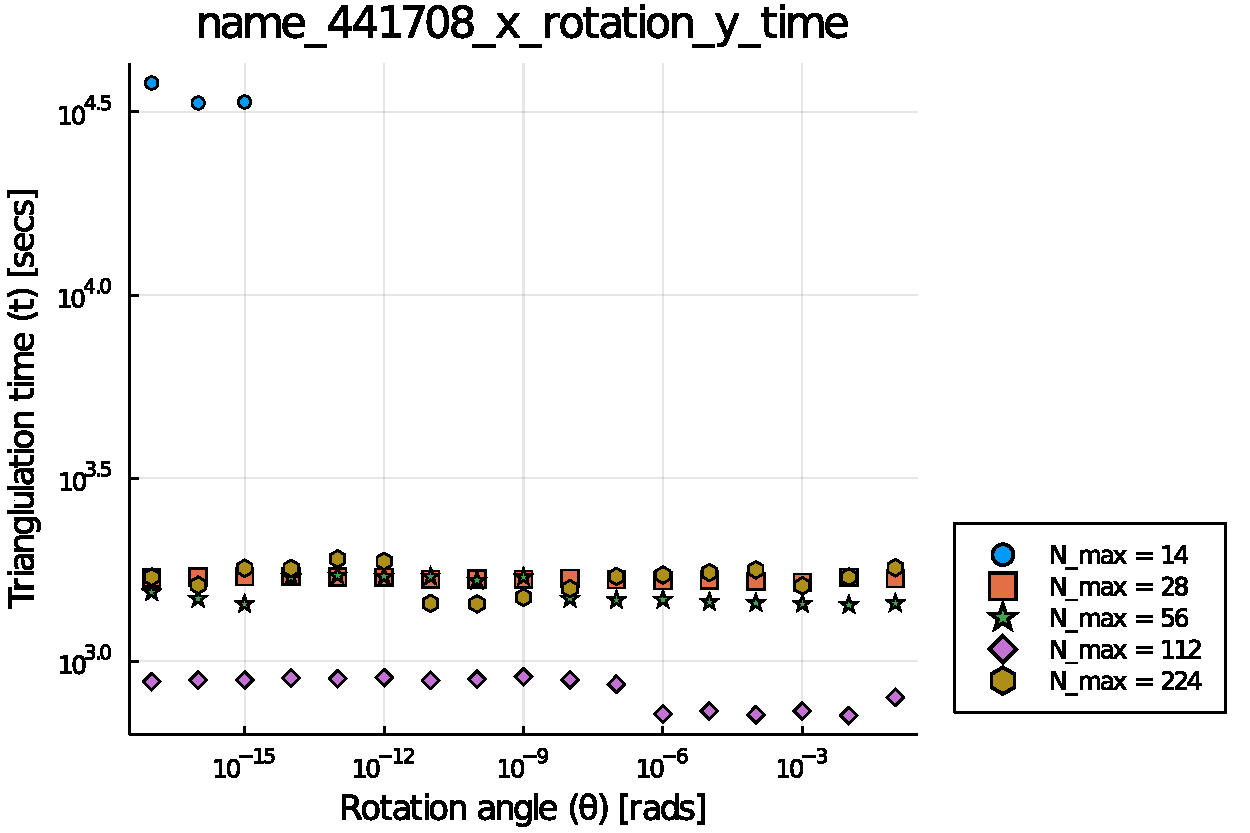
\includegraphics[width=0.95\textwidth]{../analysis/plots/name_441708_x_rotation_y_time.pdf}
  \put (-70,100) {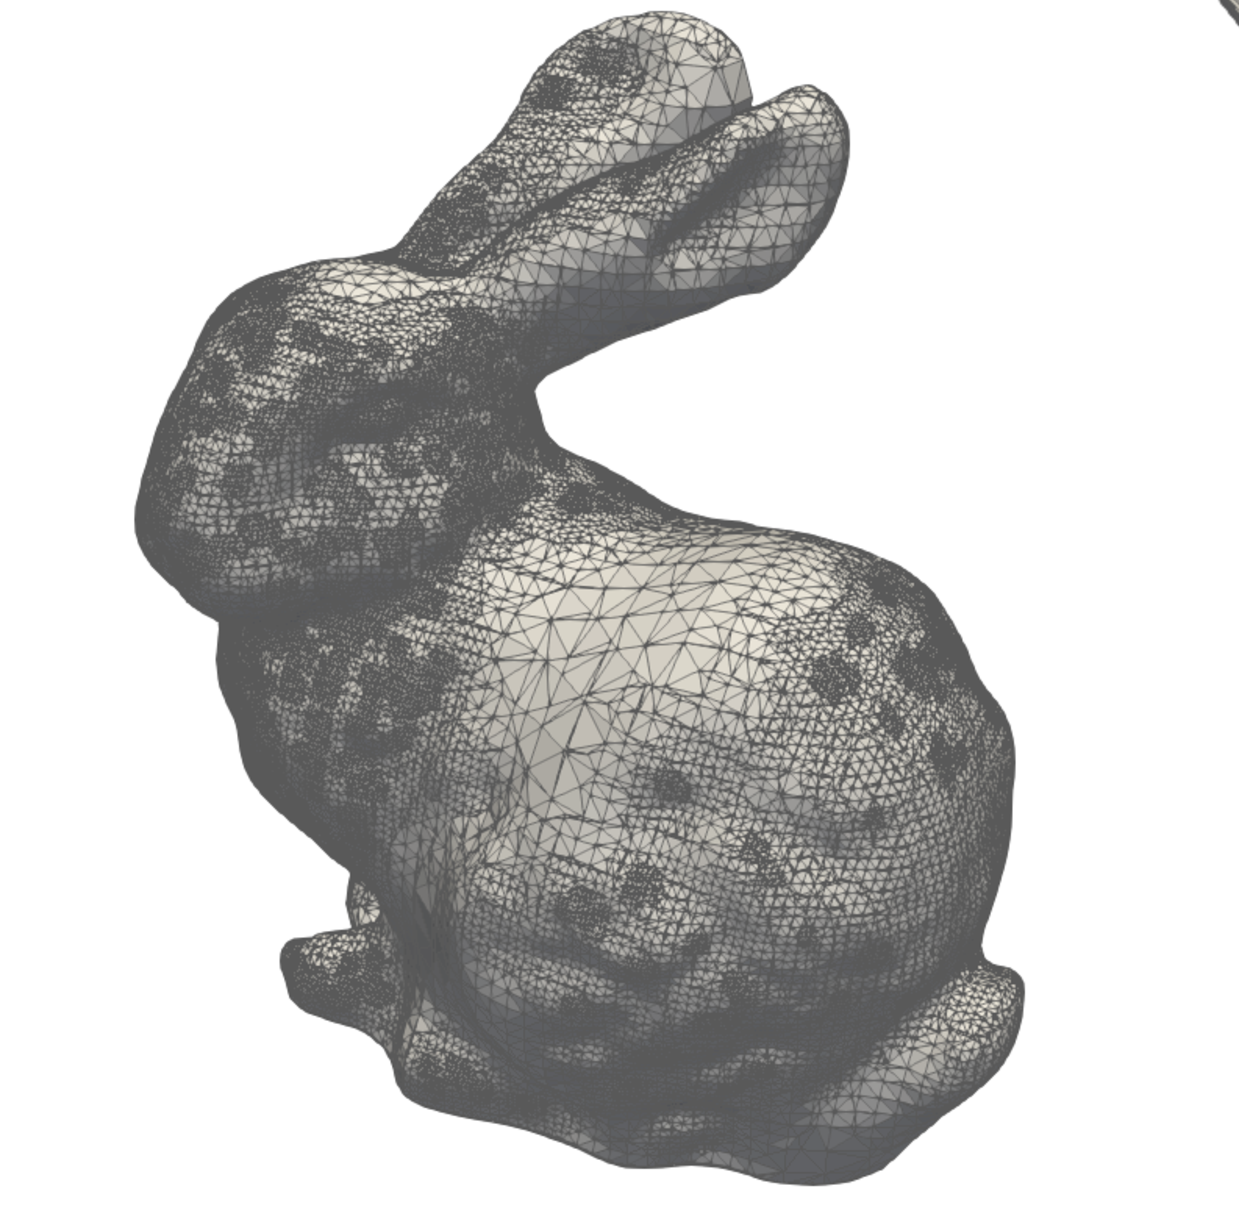
\includegraphics[width=0.2\textwidth]{441708}}
\end{frame}

\begin{frame}{Robustness matrix}
  
  \textbf{Collected results:}

  \begin{itemize}
    \item  
      \href{run:domain_volume.pdf}{Domain Volume Variation}
    \item
      \href{run:domain_surface.pdf}{Domain Surface Variation}
    \item
      \href{run:volume_error.pdf}{Domain Volume Error}
    \item
      \href{run:surface_error.pdf}{Surface Error}
    \item
      \href{run:time.pdf}{CPU time (not accurate)}
    \item
      \href{run:subcells_x_cell.pdf}{\{Min,Max,Avg\} num subcells per cell }
  \end{itemize}


\end{frame}


\begin{frame}{Conclusions and pending work}

  \textbf{Conclusion so far}
  \begin{itemize}
    \item
      Issues are depending on the geometry
    \item
      Most of problematic geometries can be found \textit{a priori}
  \end{itemize}
  \textbf{Ongoing work}
  \begin{itemize}
    \item
      Detect true degenerated geometries
    \item
      Run Gridap
  \end{itemize}


\end{frame}
\end{document}
